%!TEX root=../main.tex
\section{Empirical analysis} % (fold)
\label{sec:empirical_analysis}


Using simulated data, we compare the estimation of the eigencomponents \textcolor{red}{and the reconstruction of the curves} using the diagonalization of the covariance operator, \textcolor{red}{(a) based on univariate FPCA as well as (b) P-splines basis expansion, and (c) the diagonalization of the Gram matrix. These methods will be refered as (a) \texttt{(Tensor) PCA}, (b) \texttt{2D/1D B-Splines} and (c) \texttt{Gram} respectively. For the diagonalization of the covariance operator, we consider the methodology of \cite{happMultivariateFunctionalPrincipal2018a}. In the case of MFPCA based on the expansion of each univariate feature into univariate principal components (\texttt{(Tensor) PCA}), the eigencomposition of the 1-dimensional curves is performed using univariate FPCA and the eigendecomposition of the 2-dimensional curves is calculated using the Functional Canonical Polyadic-Tensor Power Algorithm (FCP-TPA) for regularized tensor decomposition \citep{allenMultiwayFunctionalPrincipal2013a}. In the case of MFPCA based on P-splines basis expansion (\texttt{2D/1D B-Splines}), data are expanded in B-splines basis with suitable smoothness penalty \citep{eilersFlexibleSmoothingBsplines1996}.}

The results of the simulation are compared using computation times (CT), the integrated squared error (ISE) for the multivariate eigenfunctions, the \textcolor{red}{relative squared error (RSE)} for the eigenvalues and the mean relative squared error (MRSE) for the reconstructed data. Let $\phi_k$ be the true eigenfunction and $\widehat{\phi}_k$ the estimated eigenfunction defined on $\TT{}$. We then define the ISE as 
\begin{equation}\label{eq:ise_eigenfunctions}
    \text{ISE}(\phi_k, \widehat{\phi}_k) = \normH{\phi_k - \widehat{\phi}_k}^2 = \sum_{p = 1}^P \int_{\TT{p}} \{\phi^{(p)}_k(t_p) - \widehat{\phi}^{(p)}_k(t_p)\}^2 \dd t_p, \quad k = 1, \dots, K.
\end{equation}
Let $\lambda = \{\lambda_1, \dots, \lambda_K\}$ be the set of true eigenvalues and $\widehat{\lambda} = \{\widehat{\lambda}_1, \dots, \widehat{\lambda}_K\}$ be the set of estimated eigenvalues. We then define the RSE as 
\begin{equation}\label{eq:mse_eigenvalues}
    \textcolor{red}{\text{RSE}(\lambda_k, \widehat{\lambda}_k) = \left(\lambda_k - \widehat{\lambda}_k\right)^2 / \lambda_k^2, \quad k = 1, \dots, K.}
\end{equation}
Let $\mathcal{X}$ be the set of true data and $\widehat{\mathcal{X}}$ be the set of reconstructed data. We define the MISE of the reconstructed data as
\begin{equation}\label{eq:mise_reconstructed_data}
    \text{MRSE}(\mathcal{X}, \widehat{\mathcal{X}}) = \frac{1}{N}\sum_{n = 1}^N \normH{X_n - \widehat{X}_n}^2 = \frac{1}{N}\sum_{n = 1}^N \sum_{p = 1}^P \int_{\TT{p}} \left\{\Xnp(t_p) - \hatXnp{p}(t_p) \right\}^2 \dd t_p.
\end{equation}
Each integral is approximated by the trapezoidal rule with an equidistant grid.

\subsection{Simulation experiments} % (fold)
\label{sub:simulation_experiments}

\textcolor{red}{The simulation setting is based on the \emph{Setting 3} of the simulation in \cite{happMultivariateFunctionalPrincipal2018a}.
The data generating process is based on a truncated version of the Karhunen-Loève decomposition. We simulate multivariate functional data with $P = 2$ components. For the first component, we generate an orthonormal basis $\{\phi^{(1)}_k\}_{1 \leq k \leq K}$ of $\sLp{\TT{1}}$ on an interval $\TT{1} = [0, 1] \times [0, 0.5]$ as the tensor product of the first Fourier basis functions:
\begin{equation}
    \phi^{(1)}_k(s, t) = \psi_l(s) \otimes \psi_m(t), \quad s \in [0, 1] \text{ and } t \in [0, 0.5],\quad k = 1, \dots, K,
\end{equation}
where $\psi_l$ and $\psi_m$ are elements of the Fourier basis. For the second component, we generate an orthonormal Legendre basis $\{\phi^{(2)}_k\}_{1 \leq k \leq K}$ of $\sLp{\TT{2}}$ on an interval $\TT{2} = [-1, 1]$. To ensure orthonormality, the basis $\phi^{(1)}_k$ and $\phi^{(2)}_k$ are weighted by random factors $\alpha^{1/2}$ and $(1 - \alpha)^{1/2}$, respectively, where $\alpha \sim \mathcal{U}(0.2, 0.8)$.
Each curve is then simulated using the truncated multivariate Karhunen-Loève expansion \eqref{eq:kl_multi_trunc}:
\begin{equation}
    X(\pointt) = \sum_{k = 1}^K \mathfrak{c}_k \phi_k(\pointt), \quad \pointt \in \TT{} \coloneqq \TT{1} \times \TT{2},
\end{equation}
where $\phi_k = (\phi^{(1)}_k, \phi^{(2)}_k)^\top$ and the scores $\mathfrak{c}_k$ are sampled as random normal variables with mean $0$ and variance $\lambda_k$. The eigenvalues $\lambda_k$ are defined with an exponential decrease, $\lambda_k = \exp(-(k + 1)/2)$ We simulate, for each replication of the simulation, $N = 50, 100$ and $250$ observations. The first component is sampled on a regular grid of $M^{(1)} = 11 \times 11, 26 \times 26$ and $101 \times 51$ sampling points. The second component is sampled on a regular grid of $M^{(2)} = 21, 51$ and $201$ sampling points. We set $K = 25$.}
\textcolor{red}{We also consider data with measurement errors. In that case, we observe data from \eqref{eq:model_error}, where $\sigma^2 = 0.25$. Finally, we study sparse data as in \cite{happMultivariateFunctionalPrincipal2018a}, with medium ($50\%-70\%$ missing) and high ($90\%-95\%$ missing) sparsity.}

\textcolor{red}{The \texttt{(Tensor) PCA} method is based on the univariate estimation of $K^{(1)} = 20$ eigenimages and $K^{(2)} = 15$ eigenfunctions. The estimation of the eigenimages is performed with the FCP-TPA where the smoothing parameters are chosen via cross-validation in $[10^{-5}, 10^5]$ for dense, sparse and noisy data. In the case of sparse data, we also linearly interpolate the observation to get data that are regularly sampled. The estimation of the eigenfunctions is done using the PACE algorithm \citep{yaoFunctionalDataAnalysis2005} with P-splines to smooth the mean and covariance functions. Penalties are chosen using cross-validation \citep{eilersFlexibleSmoothingBsplines1996}.}

\textcolor{red}{For the \texttt{2D/1D B-splines} method, $X^{(1)}$ is expanded in tensor products of $K^{(1)} = 13 \times 13$ B-splines and $X^{(2)}$ is expanded in $K^{(2)} = 13$ B-splines. For dense data, no penalty is involved, while for sparse and noisy data, penalties are estimated using cross-validation.}

\textcolor{red}{Finally, the \texttt{Gram} method is based on the observed data points in the dense case, on the linear interpolation of the data in the sparse case \citep{benkoCommonFunctionalPrincipal2009} and on the P-splines smoothing of the data in the noisy case.}


% subsection simulation_experiments (end)

\subsection{Simulation results} % (fold)
\label{sub:simulation_results}

We compared MFPCA results of the different methods in terms of their CT, estimation of eigenvalues (RSE), estimation of eigenfunctions (ISE), and reconstruction of curves (MRSE). We fix the number of retained components to be $12$ for each simulation scenario. Each experiment is repeated $200$ times. The results are presented below.

% Computation time ----------
\begin{results}[Computational time.]
\textcolor{red}{To compare the computational time of the different methods, we measured the time taken for each method to complete the MFPCA for each simulated dataset in the dense and noiseless case. Figure~\ref{fig:computation_time_mfd_1d} shows the kernel density estimates of the ratio of CT for each method across all sample sizes and number of sampling points. Except when we have many observations with few sampling points, the \texttt{Gram} method is faster than the other two methods. This result is coherent with the computational complexity derived in Section~\ref{sub:computational_complexity}.}
%Note that the number of features $P$ does not change the ratio of CT between the methods.

\begin{figure}
     \centering
    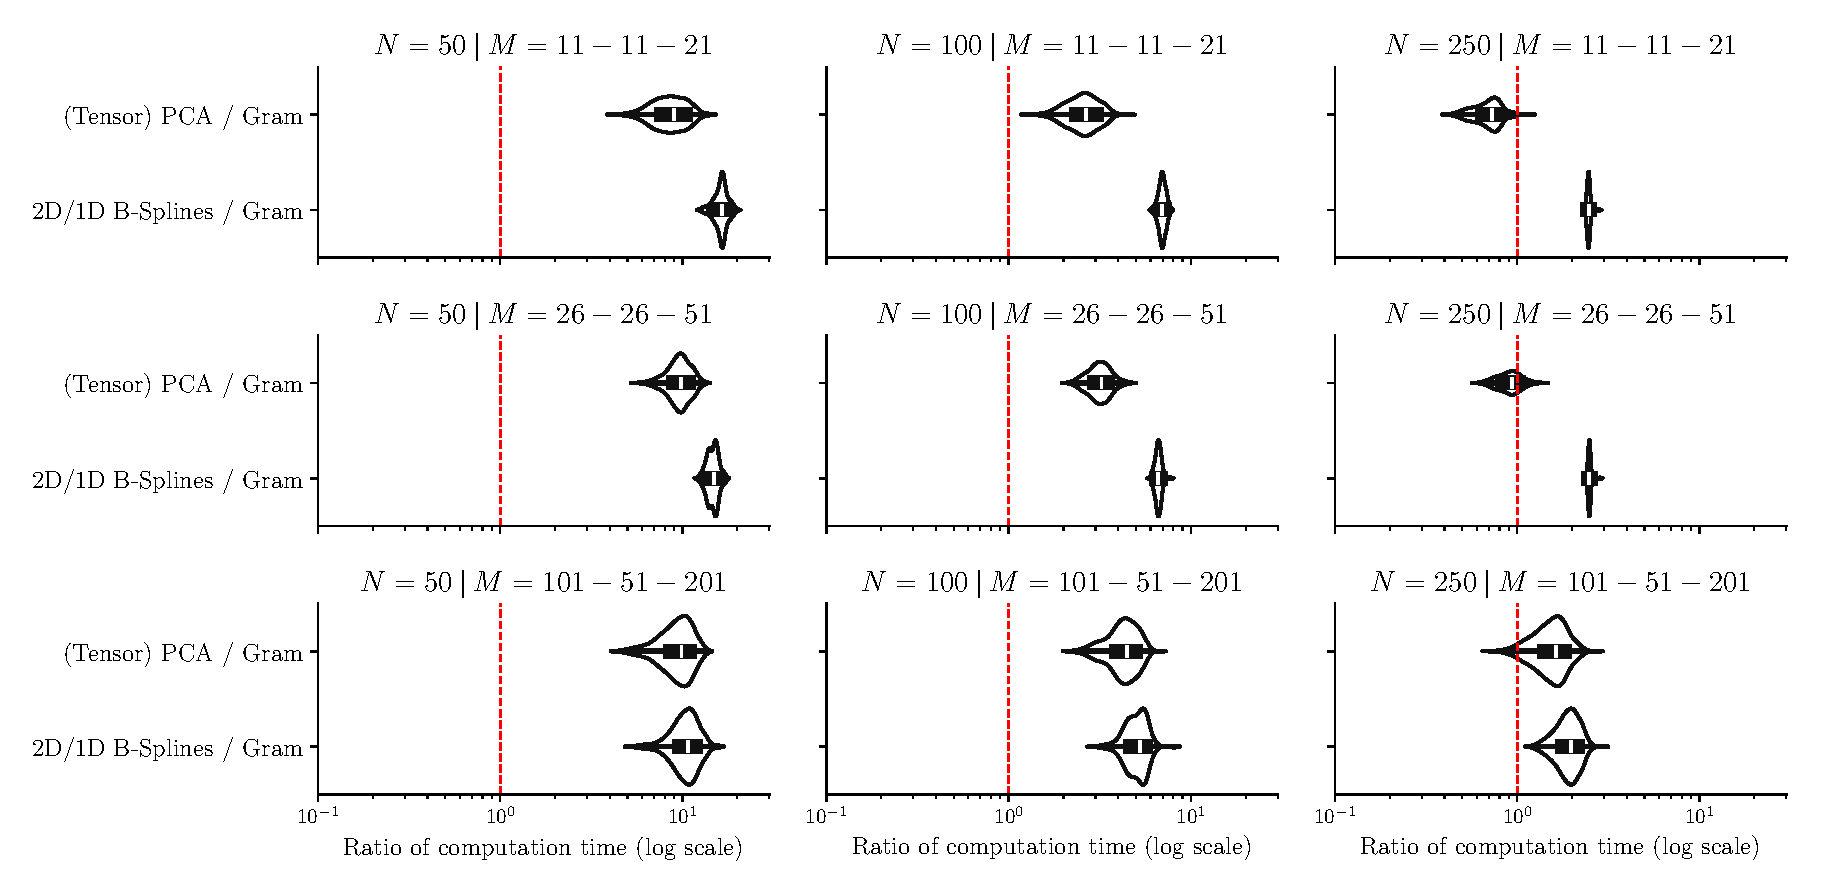
\includegraphics[width=0.95\textwidth]{figures/computation_time.eps}
    \caption{\textcolor{red}{Ratio of computation time in the dense case between the \texttt{(Tensor) PCA} and \texttt{2D/1D B-Splines} methods and the \texttt{Gram} method. $N$ is the number of observations, $M$ is the number of sampling points per curve (the first two numbers are for the images and the last one is for the curves).}}
    \label{fig:computation_time_mfd_1d}
\end{figure}

\textcolor{red}{The shorter computational time of the diagonalization of the Gram matrix makes it a more efficient option for analyzing two and higher-dimensional functional datasets as the number of sampling points tend to grow faster in these situations. It is worth noting however, that the computational time can still vary depending on the specific implementation of each method, the computational resources available, the complexity of the dataset (number of observations, number of sampling points, etc.) and whether a smoothing step need to be included.}
\end{results}

% Eigenvalues estimation ----------
\begin{results}[Eigenvalues estimation.]
\textcolor{red}{To compare the estimation of the eigenvalues between the different methods, we calculated the RSE \eqref{eq:mse_eigenvalues} between the estimated eigenvalues and the true eigenvalues for each simulated dataset and for the twelve estimated eigenvalues.
Figure~\ref{fig:logAE_mfd_1d} shows the boxplots of the RSE for each method across all sample sizes, number of sampling points. We found that the three methods behave similarly for the settings with a moderately large to a large number of sampling points. When we observe only a few sampling points, $M^{(1)} = 11 \times 11$ and $M^{(2)} = 21$, the quality of the estimation is approximately the same for the first three eigenvalues for all methods, but from the fourth eigenvalues, the \texttt{2D/1D B-splines} and the \texttt{Gram} methods give slightly better results than the \texttt{(Tensor) PCA} method. The results for the sparse and noisy cases are similar and are provided in the Appendix \ref{sub:simulation}.}

\begin{figure}
    \centering
    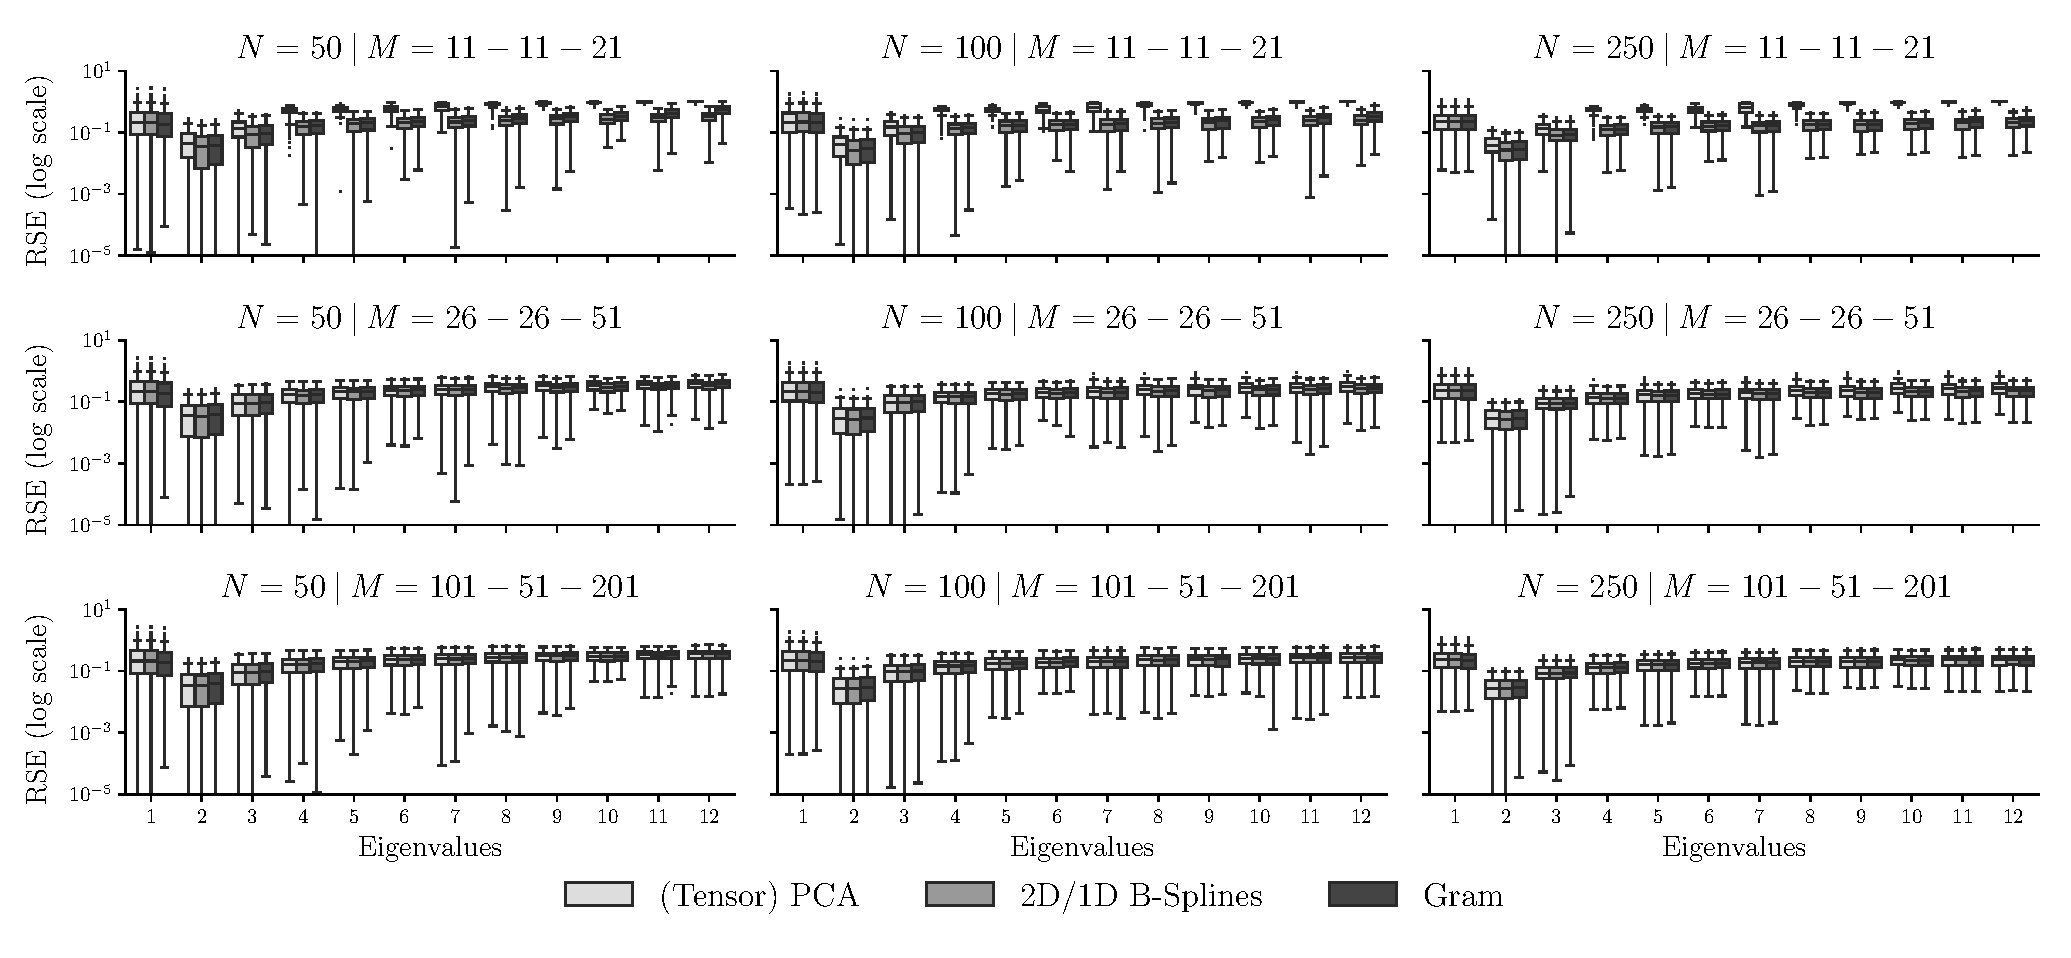
\includegraphics[width=0.95\textwidth]{figures/AE.eps}
    \caption{\textcolor{red}{RSE for the estimated eigenvalues for each method in the dense case. $N$ is the number of observations, $M$ is the number of sampling points per curve (the first two numbers are for the images and the last one is for the curves).}}
    \label{fig:logAE_mfd_1d}
\end{figure}
\end{results}

% Eigenfunctions estimation ----------
\begin{results}[Eigenfunctions estimation.]
\textcolor{red}{To compare the estimation of the eigenfunctions between the different methods, we calculated the ISE \eqref{eq:ise_eigenfunctions} between the estimated eigenfunctions and the true eigenfunctions for each simulated dataset and for the twelve estimated eigenfunctions. Figure~\ref{fig:ise_mfd_1d} shows the boxplots of the ISE for each method across all sample sizes and number of sampling points. The results are similar to those found when estimating the eigenvalues. When we observe only a few sampling points, the quality of the estimation of the eigenfunctions starts to decrease after the third component for the \texttt{(Tensor) PCA} method, while this is not the case for the other methods. The results for the sparse and noisy cases are similar and are provided in the Appendix \ref{sub:simulation}.}
\begin{figure}
     \centering
    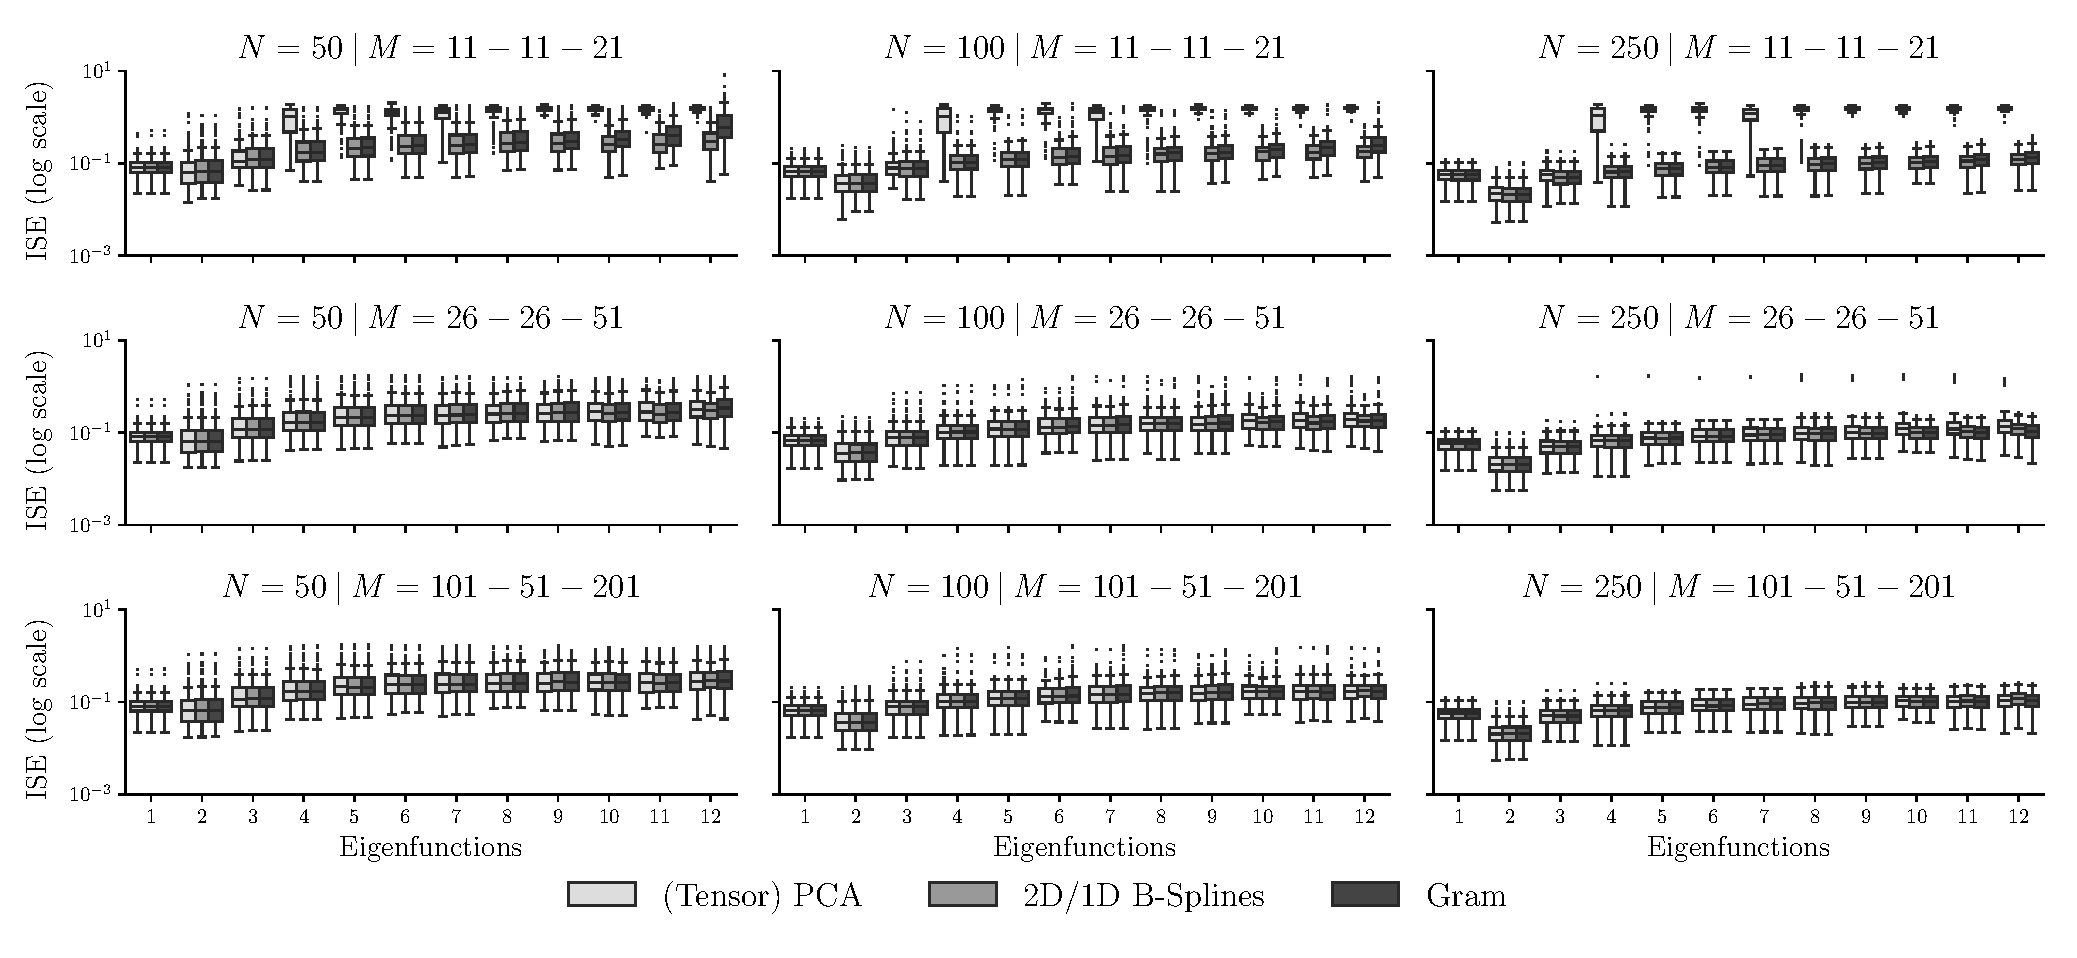
\includegraphics[width=0.95\textwidth]{figures/ISE.eps}
    \caption{\textcolor{red}{ISE for the estimated eigenfunctions for each method in the dense case. $N$ is the number of observations, $M$ is the number of sampling points per curve (the first two numbers are for the images and the last one is for the curves).}}
    \label{fig:ise_mfd_1d}
\end{figure}
\end{results}

% Curves reconstruction ----------
\begin{results}[Curves reconstruction.]
\textcolor{red}{To compare the quality of the reconstruction of the curves between the different methods, we calculated the MRSE \eqref{eq:mise_reconstructed_data} between the reconstruction of the curves and the true curves for each simulated dataset. Figure~\ref{fig:mise_mfd_1d} shows the boxplots of the MRSE for each method across all sample sizes and number of sampling points. Except in the case of few sampling points where the \texttt{(Tensor) PCA} method does not perform well (because of the poor estimation of the eigenvalues and eigenfunctions), all methods give nearly the same results for each setting. The results for the sparse and noisy cases are similar and are provided in the Appendix \ref{sub:simulation}.}
\begin{figure}
     \centering
     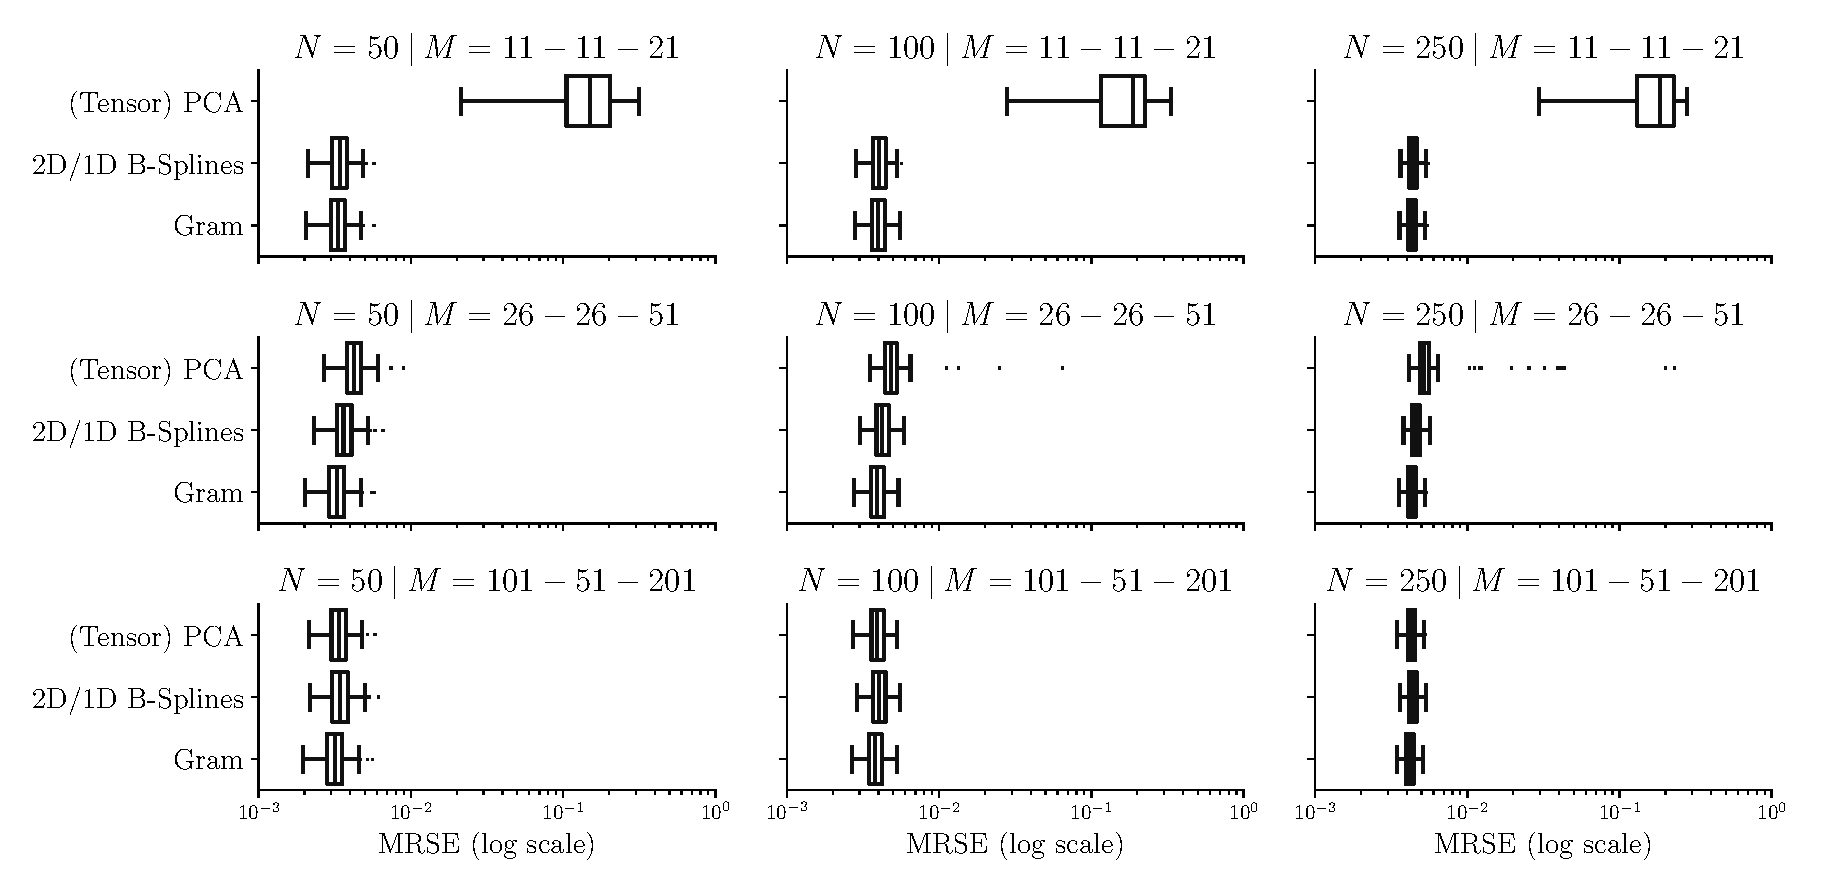
\includegraphics[width=0.95\textwidth]{figures/MRSE.eps}
    \caption{\textcolor{red}{MRSE for the reconstructed curves for each method in the dense case. $N$ is the number of observations, $M$ is the number of sampling points per curve (the first two numbers are for the images and the last one is for the curves).}}
    \label{fig:mise_mfd_1d}
\end{figure}
\end{results}


% subsection simulation_results (end)

% \subsection{Percentage of variance explained} % (fold)
% \label{sub:percentage_of_variance_explained_simulation}

% \textcolor{red}{We argue that the percentage of variance explained in \cite{happMultivariateFunctionalPrincipal2018a} is sub-optimal as they consider the variance explained by each of the components separately and not the percentage explained overall. Using the inner product matrix however gives the correct number of eigenfunctions for a given amount of variance explained.
% We also consider the estimation of the number of components to retain to reach a pre-specified percentage of variance explained by the data based on Scenario~1 with $P = 2$, $K = 20$ and we use linear and exponential decreasing of the eigenvalues. The true percentage of variance explained by the $k$th component is given by $\lambda_k / \sum_{k^\prime = 1}^{20} \lambda_{k^\prime}$ and the true percentage of variance explained by the first $K (\leq 20)$ components is given by $\sum_{k = 1}^K \lambda_k / \sum_{k^\prime = 1}^{20} \lambda_{k^\prime}$.
% Let's fix a certain percentage of variance explained $\alpha \in [0, 1]$. We define $\widetilde{K}$ as the minimum number of components required to reach $100\alpha\%$ of the variance explained,
% \begin{equation}
%     \widetilde{K} = \arg\min_K \frac{\sum_{k = 1}^K \lambda_k}{\sum_{k^\prime = 1}^{20} \lambda_{k^\prime}} \geq \alpha.
% \end{equation}
% Using the covariance operator, the implementation of \cite{happMultivariateFunctionalPrincipal2018a} does not allow for the direct estimation of $\widetilde{K}$ from multivariate functional data. They propose however to estimate the number of univariate eigenfunctions $K_1$ and $K_2$ based on the percentage of variance explained for both elements. The number of multivariate eigenfunctions is then set to be $\min\{K_1 + K_2, K\}$ where $K$ is a given scalar. To investigate the robustness of their approach, in our simulation, we first run FPCA on each univariate components to estimate the number of components needed to explain $\alpha\%$ of the variance for each component. Then, we run an MFPCA with $K = K_1 + K_2$. Using the Gram matrix, we directly estimated the number of components needed to explain a certain percentage of the variance from the multivariate functional data.
% The results shown in Figure~\textcolor{red}{...} that choosing a univariate cut-off within each dimension (e.g., $95\%$), tends to overestimate the final amount of variance – the sum of the final eigenvalues is larger than the sum of the true eigenvalues.}


% % subsection percentage_of_variance_explained (end)

% section empirical_analysis (end)